\documentclass[11pt,a4paper]{article}

% Packages
\usepackage[utf8]{inputenc}
\usepackage[margin=0.9in]{geometry}
\usepackage{graphicx}
\usepackage{hyperref}
\usepackage{fancyhdr}
\usepackage{listings}
\usepackage{xcolor}
\usepackage{titlesec}
\usepackage{enumitem}
\usepackage{float}

% Hyperref setup
\hypersetup{
    colorlinks=true,
    linkcolor=blue,
    filecolor=magenta,      
    urlcolor=cyan,
    pdftitle={Stock Strategy Backtester - Software Design Document},
    pdfpagemode=FullScreen,
}

% Code listing style
\lstset{
    backgroundcolor=\color{gray!10},
    basicstyle=\ttfamily\footnotesize,
    breaklines=true,
    frame=single,
    numbers=none,
    keywordstyle=\color{blue},
    commentstyle=\color{green!60!black},
    stringstyle=\color{red},
    showstringspaces=false,
    tabsize=2
}

% Header and footer
\pagestyle{fancy}
\fancyhf{}
\fancyhead[L]{Stock Strategy Backtester}
\fancyhead[R]{Software Design Document}
\fancyfoot[C]{\thepage}

% Title formatting - more compact
\titleformat{\section}
  {\normalfont\large\bfseries\color{blue!70!black}}{\thesection}{1em}{}
\titleformat{\subsection}
  {\normalfont\normalsize\bfseries\color{blue!50!black}}{\thesubsection}{1em}{}
  
% Reduce spacing
\titlespacing*{\section}{0pt}{8pt}{4pt}
\titlespacing*{\subsection}{0pt}{6pt}{3pt}
\setlength{\parskip}{3pt}

\begin{document}

% Title Page
\begin{titlepage}
    \centering
    \vspace*{1.5cm}
    
    {\LARGE \textbf{Stock Strategy Backtester Lite}}\\[0.3cm]
    {\Large Software Design Document}\\[0.5cm]
    {\large Digital Assignment 2}\\[1cm]
    
    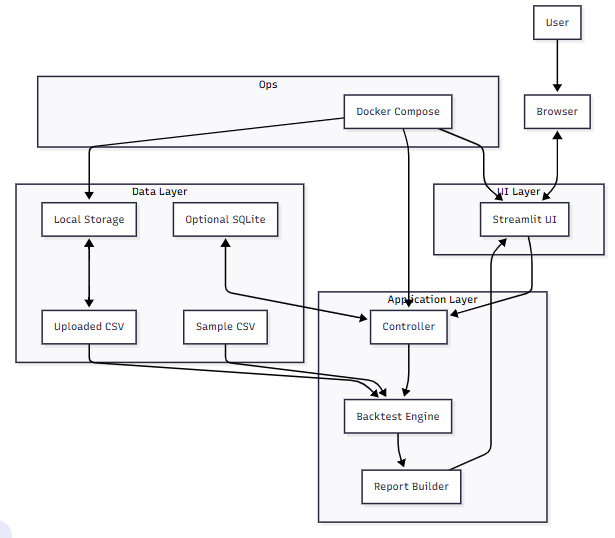
\includegraphics[width=0.55\textwidth]{diagrams/high_level_architecture.png}\\[1cm]
    
    {\normalsize Submitted by: Nihaal2004}\\[0.2cm]
    {\normalsize VIT University}\\[0.2cm]
    {\normalsize \today}\\[0.8cm]
    
    {\normalsize GitHub: \url{https://github.com/Nihaal2004/stock-backtester}}
    
    \vfill
\end{titlepage}

\section{Executive Summary}

The \textbf{Stock Strategy Backtester Lite} is an educational tool designed to help beginners evaluate trading strategies using historical stock data. The application provides a simple interface for uploading CSV data, selecting strategies (SMA Crossover, RSI Threshold), and generating performance reports including equity curves, metrics, and trade logs.

\subsection{Project Goals}
This project demonstrates professional software engineering through:
\begin{itemize}[leftmargin=*, itemsep=0pt]
    \item \textbf{Modular Design:} 6 independent modules with clear responsibilities
    \item \textbf{Design Patterns:} Strategy and Factory patterns for extensibility
    \item \textbf{Layered Architecture:} Separation between UI, business logic, and data
    \item \textbf{Best Practices:} Abstraction, high cohesion, low coupling
\end{itemize}

\subsection{Key Features}
\begin{itemize}[leftmargin=*, itemsep=0pt]
    \item Upload CSV files with historical stock data
    \item Run two strategies: SMA Crossover and RSI Threshold
    \item Visualize equity curves and performance metrics
    \item Next-day execution to prevent lookahead bias
    \item Clear error messages and validation
    \item Docker deployment for easy setup
\end{itemize}

\section{Design Principles Applied}

\subsection{Abstraction}
\textbf{Implementation:} Abstract Strategy base class defines interface for all trading strategies, hiding implementation details.

\begin{lstlisting}[language=Python]
class Strategy(ABC):
    @abstractmethod
    def generate_signals(self, df, params):
        pass  # Concrete strategies implement this

class SMAStrategy(Strategy):
    def generate_signals(self, df, params):
        # Implementation hidden from users
        return df
\end{lstlisting}

\textbf{Benefits:} UI works with abstractions; easy to add strategies without modifying existing code.

\subsection{Modularity}
\textbf{Implementation:} System divided into 6 independent modules:

\begin{table}[H]
\small
\centering
\begin{tabular}{|l|p{4cm}|p{3cm}|}
\hline
\textbf{Module} & \textbf{Responsibility} & \textbf{Key Classes} \\
\hline
data\_loader.py & Data handling & DataLoader \\
\hline
strategies.py & Trading algorithms & Strategy, SMAStrategy, RSIStrategy \\
\hline
backtest\_engine.py & Backtest execution & BacktestEngine \\
\hline
visualization.py & Charts and display & Visualizer \\
\hline
ui\_components.py & UI elements & UIComponents \\
\hline
app.py & Orchestration & main() \\
\hline
\end{tabular}
\end{table}

\textbf{Benefits:} Independent development, testing, and maintenance; changes don't cascade.

\subsection{High Cohesion}
\textbf{Implementation:} Each module has single, well-defined purpose. Example: DataLoader handles all data operations (load, validate, clean, filter).

\textbf{Benefits:} Easy to understand; reduces complexity; simplifies testing.

\subsection{Low Coupling}
\textbf{Implementation:} Modules communicate through standard interfaces (DataFrames, dictionaries). BacktestEngine doesn't know about specific strategies; UI doesn't know algorithm details.

\textbf{Benefits:} Changes in one module don't affect others; modules can be reused.

\subsection{Design Patterns Used}

\subsubsection{Strategy Pattern}
Allows selecting trading algorithms at runtime without modifying code.

\begin{lstlisting}[language=Python]
# Factory creates strategies dynamically
class StrategyFactory:
    _strategies = {
        'SMA Crossover': SMAStrategy,
        'RSI Threshold': RSIStrategy
    }
    
    @classmethod
    def create_strategy(cls, name):
        return cls._strategies[name]()
\end{lstlisting}

\textbf{Benefits:} Easy to add new strategies; UI doesn't depend on strategy classes; promotes Open/Closed Principle.

\subsubsection{Factory Pattern}
Centralizes object creation and decouples UI from implementations.

\textbf{Example Usage:}
\begin{lstlisting}[language=Python]
# UI code - no knowledge of strategy classes
strategy = StrategyFactory.create_strategy("SMA Crossover")
signals = strategy.generate_signals(data, params)
\end{lstlisting}

\textbf{Benefits:} One place to manage strategies; easy to add/remove options; loose coupling.

\section{High-Level Architecture}

\subsection{Architecture Style: Layered Architecture}

The application follows a \textbf{3-layer architecture}:

\begin{figure}[H]
    \centering
    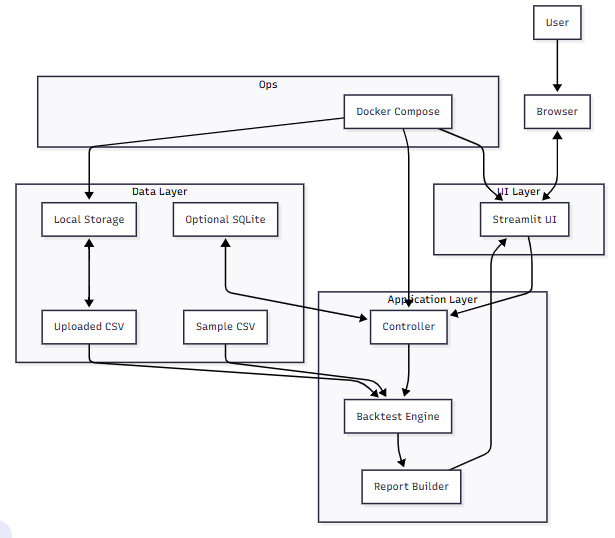
\includegraphics[width=0.75\textwidth]{diagrams/high_level_architecture.png}
    \caption{High-Level System Architecture}
\end{figure}

\textbf{Layer 1 - Presentation:} UI components and visualization (app.py, ui\_components.py, visualization.py)

\textbf{Layer 2 - Business Logic:} Trading strategies and backtesting (strategies.py, backtest\_engine.py)

\textbf{Layer 3 - Data:} Data loading and validation (data\_loader.py)

\subsection{Why Layered Architecture?}

\begin{enumerate}[leftmargin=*, itemsep=0pt]
    \item \textbf{Clear Separation:} Each layer has distinct responsibility
    \item \textbf{Standard Pattern:} Well-understood industry approach
    \item \textbf{Perfect Fit:} Matches data pipeline (load → process → display)
    \item \textbf{Maintainable:} Changes in one layer don't affect others
\end{enumerate}

\subsection{Data Flow}
The backtest execution follows a clear pipeline:

\begin{enumerate}[leftmargin=*, itemsep=0pt]
    \item \textbf{Data Layer:} User uploads CSV → DataLoader validates and cleans
    \item \textbf{Business Layer:} User selects strategy → StrategyFactory creates instance → Strategy generates signals → BacktestEngine simulates trades
    \item \textbf{Presentation Layer:} Visualizer displays equity curve, metrics, and trade log
\end{enumerate}

\begin{figure}[H]
    \centering
    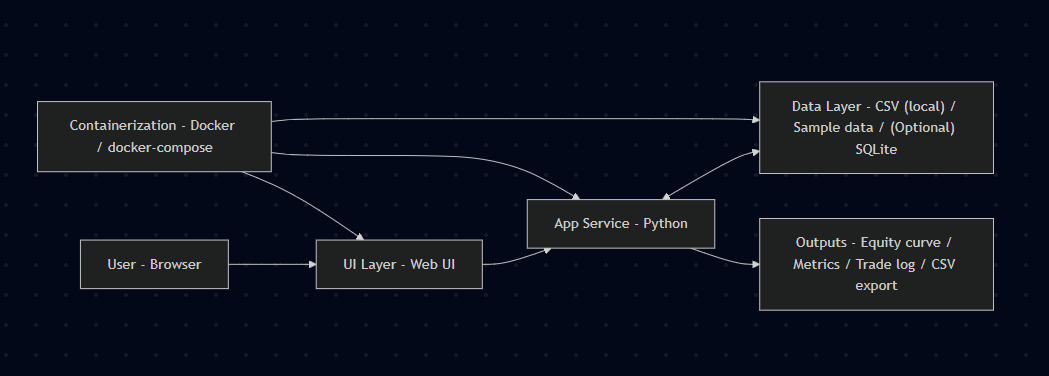
\includegraphics[width=0.8\textwidth]{diagrams/Architecture.png}
    \caption{Detailed Component Architecture}
\end{figure}

\begin{figure}[H]
    \centering
    \includegraphics[width=0.75\textwidth]{diagrams/backtest_pipline.png}
    \caption{Backtest Execution Pipeline}
\end{figure}

\subsection{Module Interactions}
\textbf{app.py} (Orchestrator) coordinates workflow:
\begin{itemize}[leftmargin=*, itemsep=0pt]
    \item Calls UIComponents to display forms
    \item Uses DataLoader to load and validate CSV
    \item Requests StrategyFactory to create strategy
    \item Passes data to BacktestEngine for simulation
    \item Invokes Visualizer to display results
\end{itemize}

\textbf{Key Design Choice:} App.py is thin—just coordination. All logic is in specialized modules.

\section{User Interface Design}

\subsection{Design Philosophy}
Simplicity, clarity, consistency, and user-friendly interface with step-by-step workflow.

\subsection{UI Screens}

\begin{figure}[H]
    \centering
    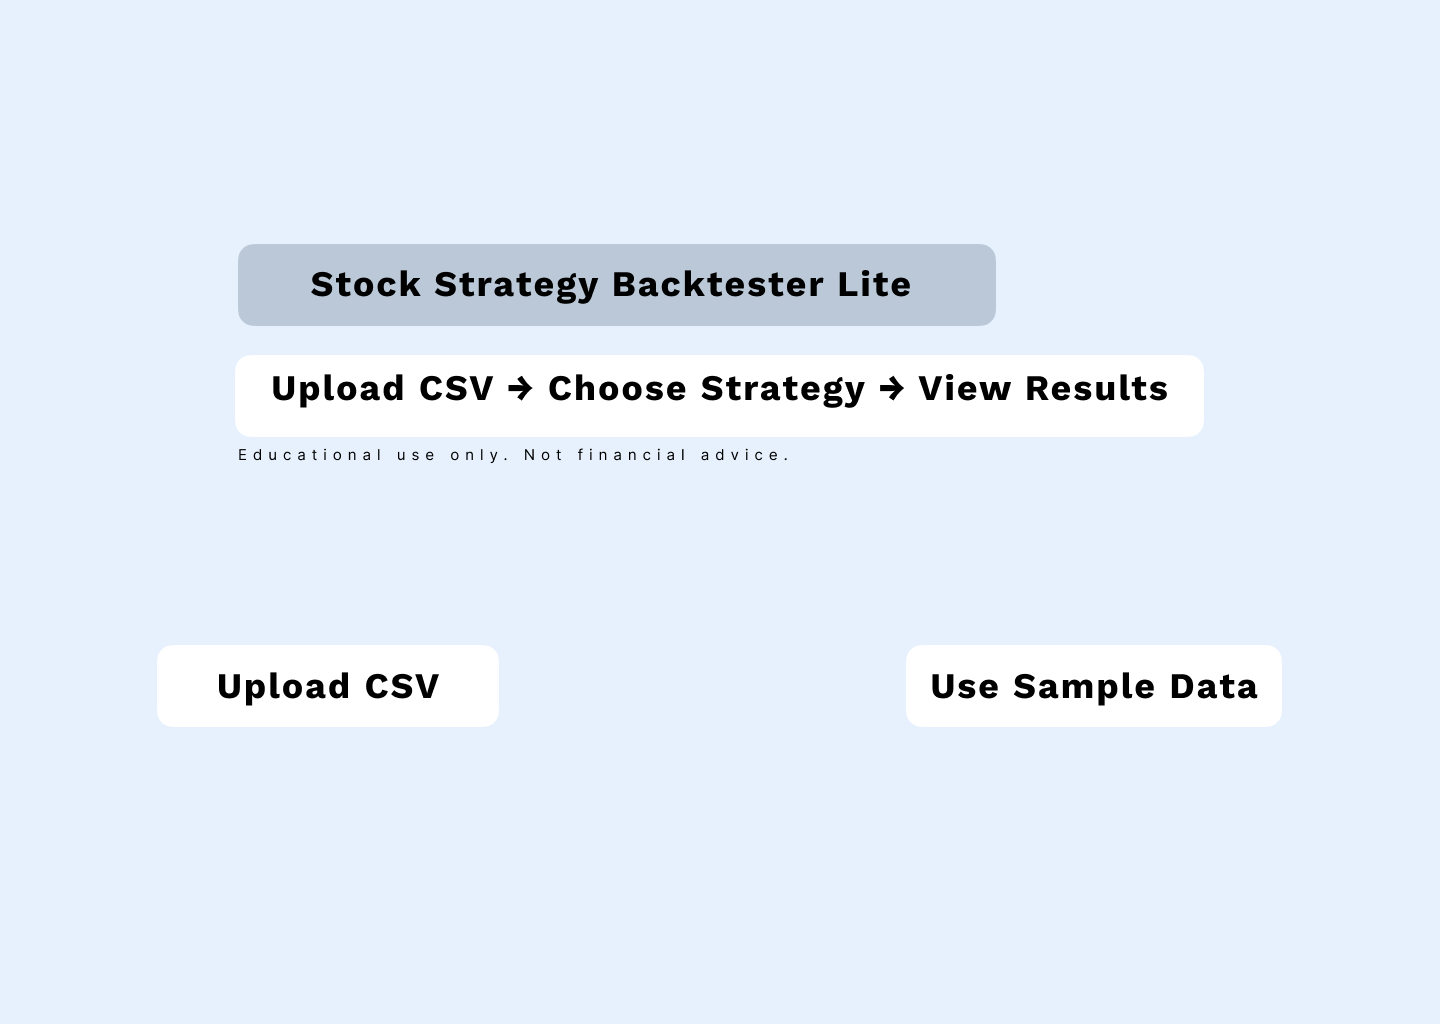
\includegraphics[width=0.5\textwidth]{wireframes/home.png}
    \caption{Home Screen - Welcome and instructions}
\end{figure}

\begin{figure}[H]
    \centering
    \begin{minipage}{0.48\textwidth}
        \centering
        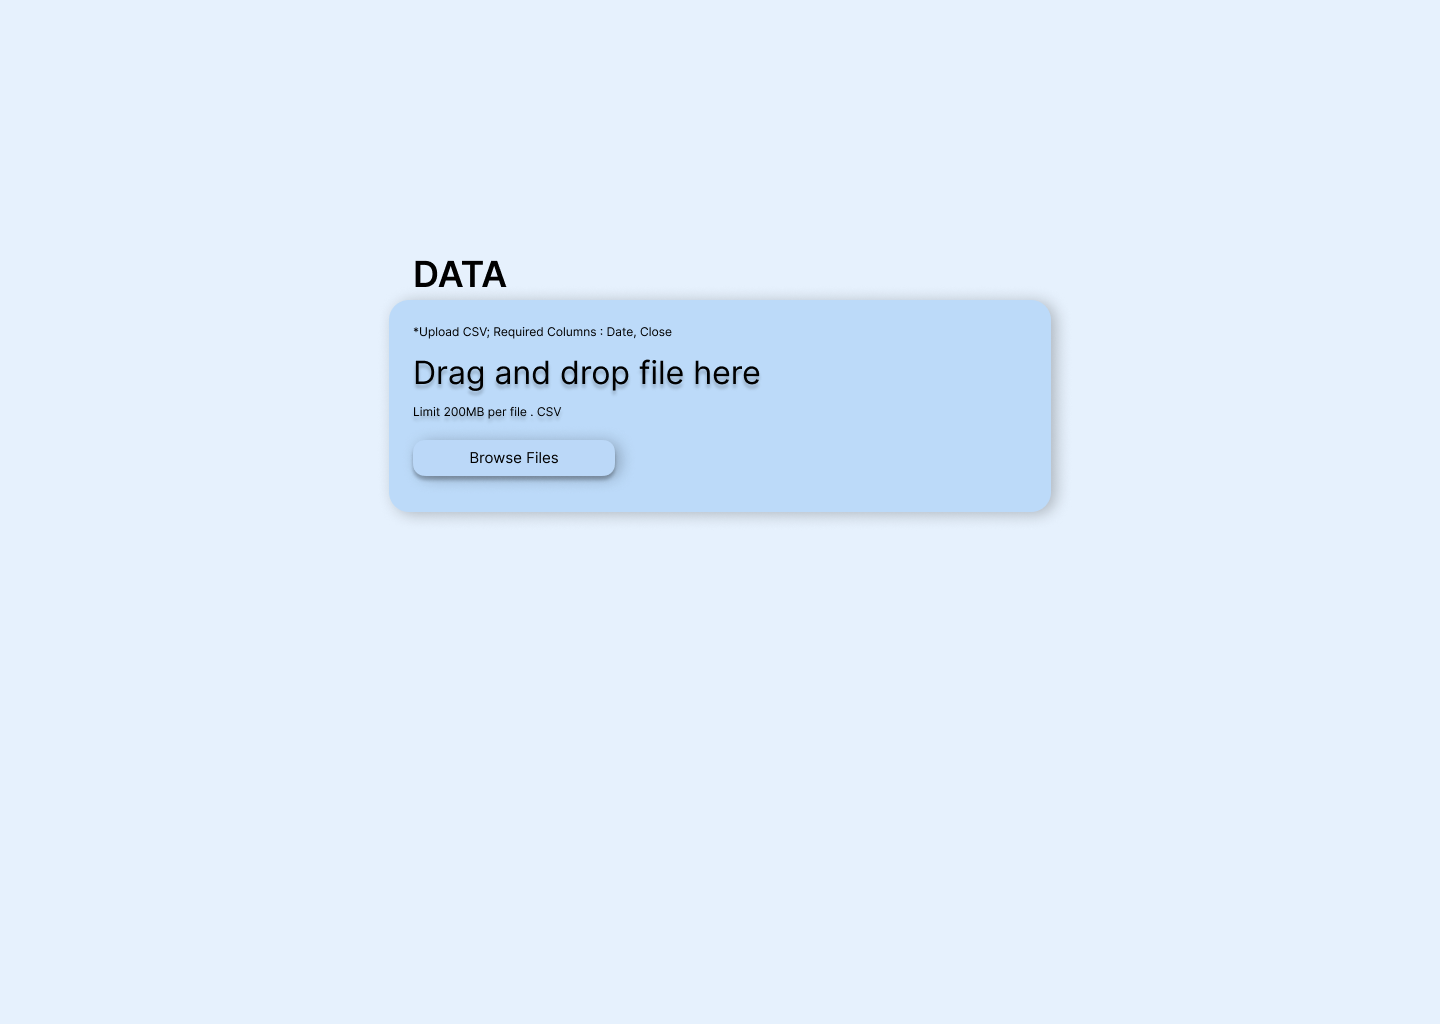
\includegraphics[width=\textwidth]{wireframes/csv_import.png}
        \caption{CSV Import - File upload}
    \end{minipage}\hfill
    \begin{minipage}{0.48\textwidth}
        \centering
        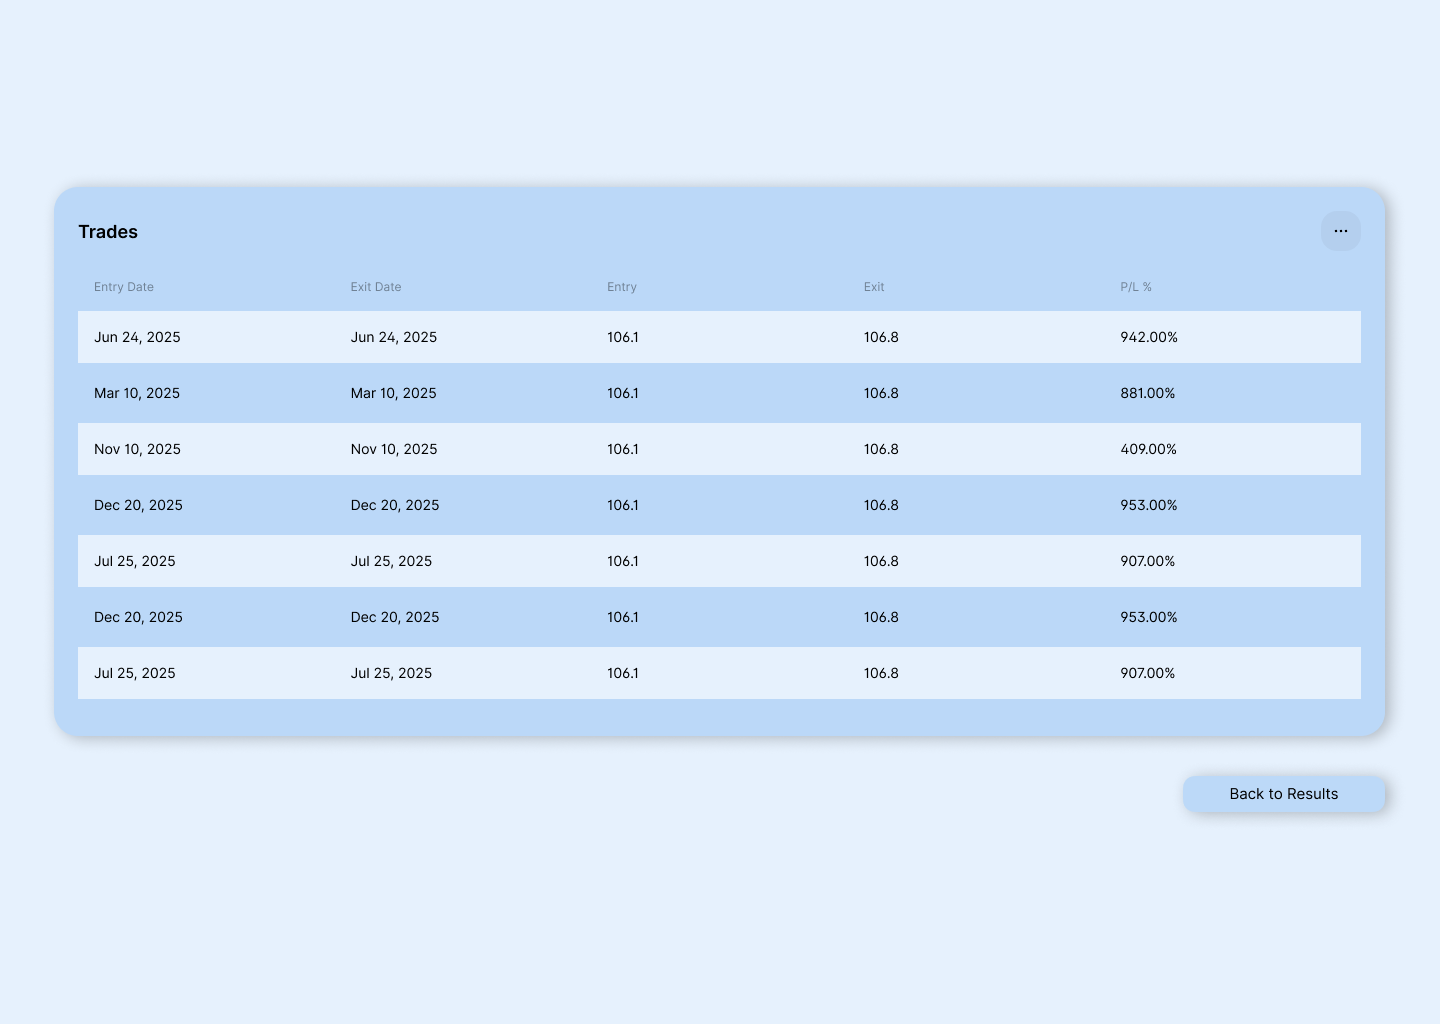
\includegraphics[width=\textwidth]{wireframes/stock_preview.png}
        \caption{Data Preview - Validation}
    \end{minipage}
\end{figure}

\begin{figure}[H]
    \centering
    \begin{minipage}{0.48\textwidth}
        \centering
        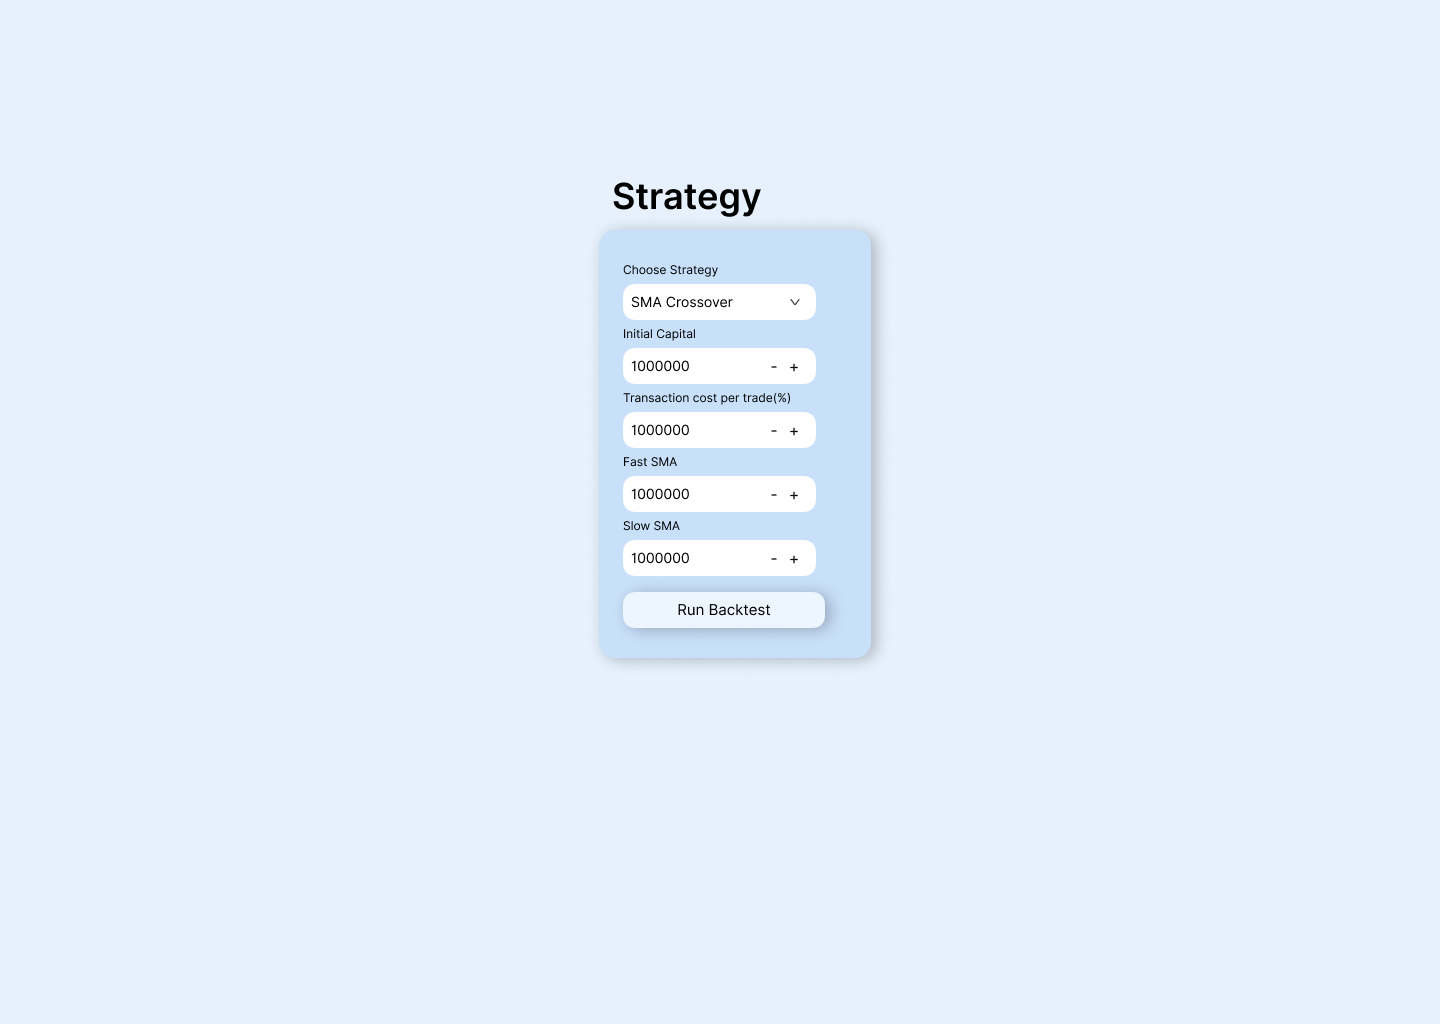
\includegraphics[width=\textwidth]{wireframes/strategy_picker.png}
        \caption{Strategy Selection - Configuration}
    \end{minipage}\hfill
    \begin{minipage}{0.48\textwidth}
        \centering
        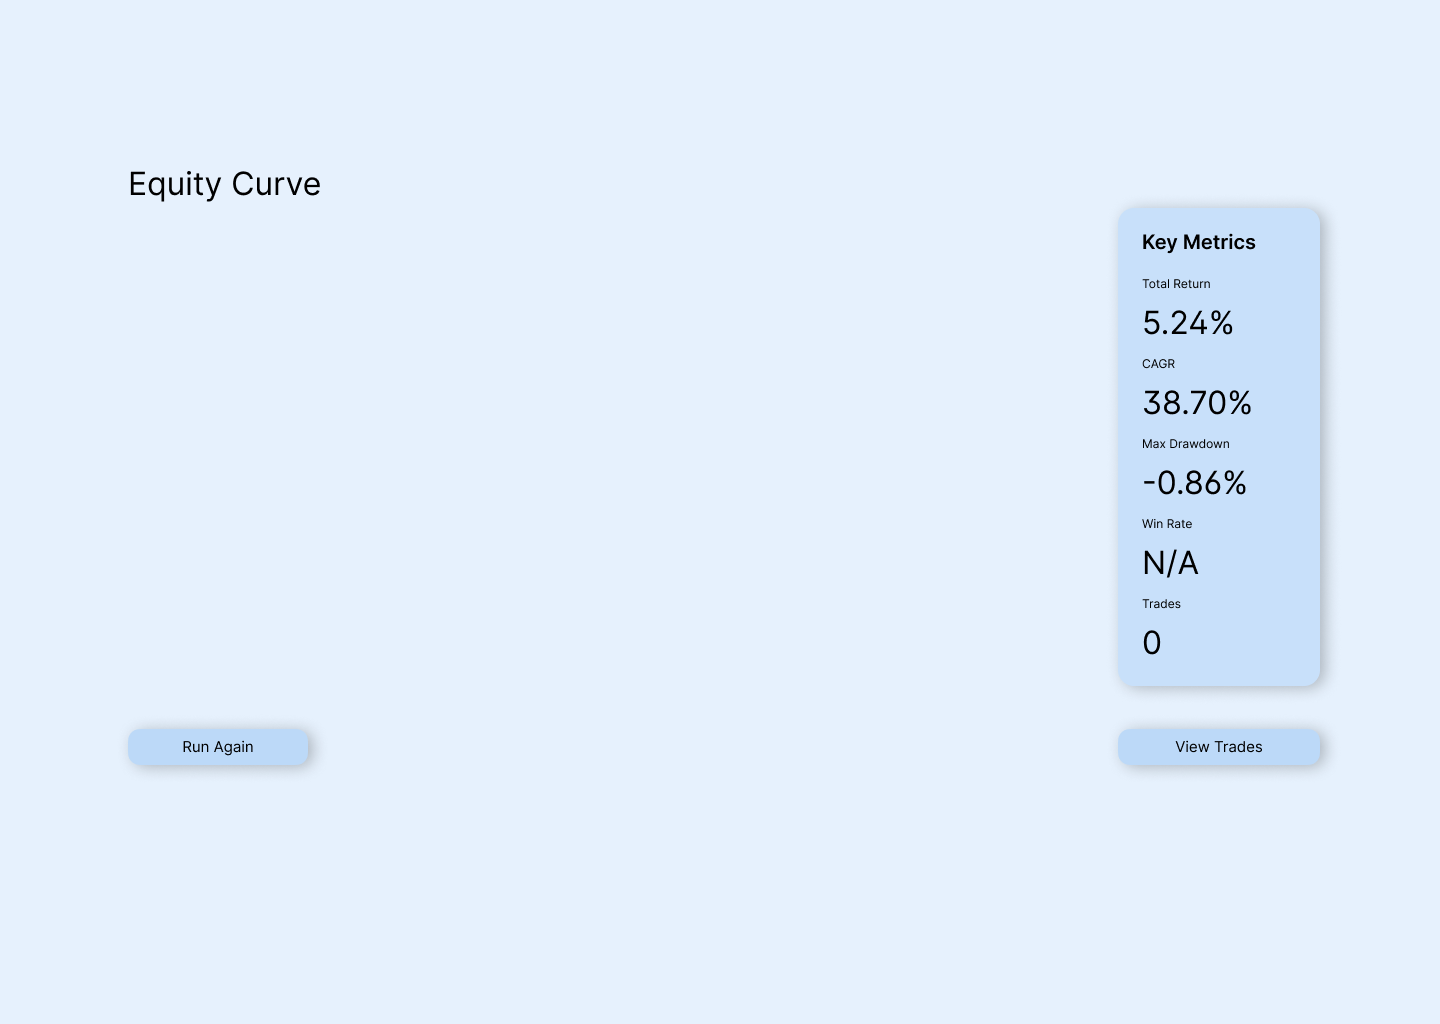
\includegraphics[width=\textwidth]{wireframes/equity_curve.png}
        \caption{Results - Equity curve and metrics}
    \end{minipage}
\end{figure}

\subsection{User-Friendly Features}
\textbf{Consistency:} Uniform colors, fonts, button styles throughout the application.

\textbf{Clarity:} Numbered steps (1️⃣, 2️⃣, 3️⃣) guide users through workflow.

\textbf{Feedback:} Loading spinners, success/error messages with clear instructions.

\textbf{Validation:} Real-time input validation with helpful error messages.

\textbf{Figma Prototype:} \url{https://www.figma.com/design/9AgSClvrB4onGZlJ19ogbf/nihaal}

\section{Design Decisions \& Rationale}

\subsection{Decision 1: Modular Architecture}
\textbf{Decision:} Refactor into 6 independent modules vs. monolithic file.

\textbf{Why:} Original 200+ line file was difficult to maintain; mixed responsibilities made testing hard.

\textbf{Alternative Rejected:} Keep in one file - poor maintainability, violates Single Responsibility.

\textbf{Outcome:} Clear separation; each module independently testable.

\subsection{Decision 2: Strategy Pattern}
\textbf{Decision:} Use abstract Strategy base class with concrete implementations.

\textbf{Why:} Easy to add new strategies without modifying existing code (Open/Closed Principle).

\textbf{Alternative Rejected:} If/else statements - hard to extend, violates design principles.

\textbf{Outcome:} New strategies added in ~15 minutes without touching existing code.

\subsection{Decision 3: Factory Pattern}
\textbf{Decision:} Centralize strategy creation in StrategyFactory.

\textbf{Why:} UI doesn't need to know about strategy classes; one place to manage all strategies.

\textbf{Alternative Rejected:} Direct instantiation - tight coupling between UI and strategies.

\textbf{Outcome:} Decoupled UI from strategy implementations.

\subsection{Decision 4: Layered Architecture}
\textbf{Decision:} 3-layer architecture (Presentation, Business Logic, Data).

\textbf{Why:} Better fit for data pipeline workflow; simpler than MVC for this use case.

\textbf{Alternative Rejected:} MVC pattern - overkill, more complex than needed.

\textbf{Outcome:} Appropriate complexity; clear structure; easy to understand.

\subsection{Decision 5: Next-Day Execution}
\textbf{Decision:} Execute trades day after signal (position today = signal from yesterday).

\textbf{Why:} Prevents lookahead bias; realistic (can't trade on today's close); professional standard.

\textbf{Alternative Rejected:} Same-day execution - unrealistic, inflates performance.

\textbf{Outcome:} Realistic backtest results; educational value.

\subsection{Additional Design Choices}

\textbf{DataFrame Communication:} Use Pandas DataFrames as standard interface between modules. Flexible, industry-standard, easy to extend.

\textbf{Clear Error Messages:} Provide detailed, actionable errors with suggestions (e.g., "Fast SMA must be less than Slow SMA. Try Fast=5, Slow=20"). Improves user experience and educational value.

\textbf{Form-Based UI:} Use explicit "Run Backtest" button instead of auto-run. Gives users control and prevents wasteful recomputation.

\textbf{Long-Only Strategy:} Support only long positions for simplicity. Appropriate for educational scope; can be extended later.

\textbf{Docker Deployment:} Package application in Docker for consistent environment. Easy setup: \texttt{docker compose up --build}.

\section{Conclusion}

This project successfully demonstrates professional software design principles applied to create maintainable, extensible code. The modular architecture with 6 independent modules, implementation of Strategy and Factory patterns, and layered architecture provide a solid foundation.

\subsection{Key Achievements}
\begin{itemize}[leftmargin=*, itemsep=0pt]
    \item \textbf{Abstraction:} Strategy base class hides implementation details
    \item \textbf{Modularity:} 6 focused modules with single responsibilities
    \item \textbf{High Cohesion:} Related functionality grouped together
    \item \textbf{Low Coupling:} Modules communicate through standard interfaces
    \item \textbf{Extensibility:} New strategies added in ~15 minutes
\end{itemize}

\subsection{Impact}
\textbf{Before Refactoring:} 200+ line monolithic file, difficult to test, hard to extend.

\textbf{After Refactoring:} 6 focused modules (~500 lines total), independently testable, easy to add features.

\textbf{Measurable Improvement:} Time to add new strategy reduced from 2-3 hours to 15 minutes.

\subsection{Design Quality}
The design prioritizes simplicity, maintainability, and educational value while following industry best practices. Clear separation of concerns makes the codebase easy to understand and modify. Design patterns (Strategy, Factory) provide proven solutions to common problems.

\subsection{Future Extensibility}
The architecture supports easy additions:
\begin{itemize}[leftmargin=*, itemsep=0pt]
    \item New strategies: Implement Strategy interface, register in Factory
    \item New metrics: Add to BacktestEngine.calculate\_metrics()
    \item Transaction costs: Add commission parameter to BacktestEngine
    \item Multiple assets: Modify DataLoader to handle multiple files
\end{itemize}

\subsection{Repository \& Resources}
\textbf{GitHub Repository:} \url{https://github.com/Nihaal2004/stock-backtester}

\textbf{Complete Documentation:} Available in \texttt{/docs/design/} folder

\textbf{Figma UI Prototype:} \url{https://www.figma.com/design/9AgSClvrB4onGZlJ19ogbf/nihaal}

\textbf{Quick Start:}
\begin{lstlisting}[language=bash]
docker compose up --build
# Access at http://localhost:8501
\end{lstlisting}

\end{document}
